\chapter{提案手法}
\label{proposed}

本章では提案手法について述べる.

\section{概要}
本研究では機材の都合上映像からの自己位置推定,機体コントロールの計算処理を遠隔PC上で行う.

全体のシステム構成は以下の図~\ref{fig:all_struct}の通りである.
\begin{figure}[htbp]
  \begin{center}
    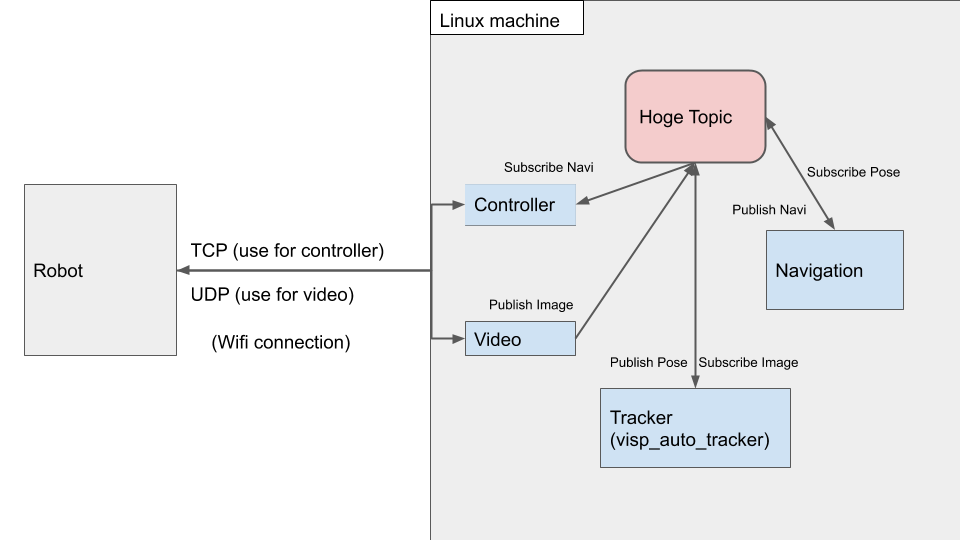
\includegraphics[clip,width=15.0cm]{img/all_struct.png}
    \caption{システム概要図}
    \label{fig:all_struct}
  \end{center}
\end{figure}

本研究ではROSの使用を前提としたシステム設計となっている.

\section{コントローラ部}
\label{implement_controller}

\begin{lstlisting}[caption=controller.py,label=go_to_target_method]
def go_to_target(self):
  print('target pos: ', self.target_pos)
  print('self pos: ', self.drone_pos) 
  move_x_val = int(self.target_pos["x"] - self.drone_pos["x"] - (self.QR_SIZE/2))
  move_y_val = int(self.target_pos["y"] - self.drone_pos["y"] - (self.QR_SIZE/2))
  move_z_val = int(self.target_pos["z"] - self.drone_pos["z"])
  rotate_val = int(self.target_pos["rotate"] - self.drone_pos["r"])
  self.is_moving = True
  if move_x_val > 0:
      self.drone.move_right(move_x_val)
      time.sleep(move_x_val/10 + self.COMMAND_WAIT_BUFFER)
      print('sleep x: ', move_x_val/10 + self.COMMAND_WAIT_BUFFER)
  else:
      self.drone.move_left(-move_x_val)
      time.sleep(-move_x_val/10 + self.COMMAND_WAIT_BUFFER)
      print('sleep x: ', -move_x_val/10 + self.COMMAND_WAIT_BUFFER)

  if move_y_val > 0:
      self.drone.move_down(move_y_val)
      time.sleep(move_y_val/10 + self.COMMAND_WAIT_BUFFER)
      print('sleep y: ', move_y_val/10 + self.COMMAND_WAIT_BUFFER)
  else:
      self.drone.move_up(-move_y_val)
      time.sleep(-move_y_val/10 + self.COMMAND_WAIT_BUFFER)
      print('sleep y: ', -move_y_val/10 + self.COMMAND_WAIT_BUFFER)

  if move_z_val > 0:
      self.drone.move_forward(move_z_val)
      time.sleep(move_z_val/10 + self.COMMAND_WAIT_BUFFER)
      print('sleep z: ', move_z_val/10 + self.COMMAND_WAIT_BUFFER)
  else:
      self.drone.move_backward(-move_z_val)
      time.sleep(-move_z_val/10 + self.COMMAND_WAIT_BUFFER)
      print('sleep z: ', -move_z_val/10 + self.COMMAND_WAIT_BUFFER)

  if rotate_val > 0:
      self.drone.rotate_cw(rotate_val)
  else:
      self.drone.rotate_ccw(-rotate_val)
  time.sleep(self.COMMAND_WAIT_BUFFER)
  self.is_moving = False
  self.is_standby = False
  self.drone_pos_list = []
  self.drone_rotate_list = []
  return
\end{lstlisting}

\section{映像システム}
\label{implement_video}

映像システムについて書く
ドローンの映像をパブリッシュする.

\section{トラッカーシステム}
\label{proposed_tracker}
トラッキングシステムについて書く

visp\_auto\_trackerの説明を書く

こいつがPnP問題諸々をやってくれる

\section{ナビゲーション部}
\label{implement_navigation}

QRコードから得られたカメラの情報と次点のQRコードの位置情報を元にドローンに対してメッセージを送信する.



%%% Local Variables:
%%% mode: japanese-latex
%%% TeX-master: "../bthesis"
%%% End:
